\begin{pastexam}[label={px:ntu-107-dsa-04}]{臺大資工所 107 學年度 第 IV 題}
（單選；答錯倒扣當題分數）

(10 points) Suppose we want to use trees to store the following 10 elements, inserted in this
exact sequence: $88,93,76,50,46,3,32,85,30,95$.
\begin{enumerate}[label=\textbf{\arabic*.}, start=13]
\item (2 points) What is the height of the tree if we insert these 10 elements in sequence into a
Binary Search Tree? (A) 4 (B) 6 (C) 7 (D) 8.
\item (2 points) In the Binary Search Tree from the previous question, suppose we remove the node
with value 76, what's the parent of the node with value 50? (A) 46 (B) 85 (C) 88 (D) 93.
\item (3 points) Suppose we insert these 10 elements in sequence into an AVL Tree, what's value of
the parent of the node with value 76? (A) 46 (B) 85 (C) 88 (D) 93.
\item (3 points) In the AVL tree from the previous question, suppose we remove the node with value
32, what's the parent of the node with value 30? (A) 3 (B) 46 (C) 50 (D) 76.
\end{enumerate}
\end{pastexam}

\begin{pastsoln}
答案：13.~(B) 6\quad 14.~(B) 85\quad 15.~(C) 88\quad 16.~(C) 50。

第 13、14 題的答案取決於兩個慣例，先說明：高度照 CLRS 數\textbf{邊}（和第 II 題同一份考卷）；刪除
有兩個子節點的節點時，用\textbf{後繼}（右子樹最小）取代，這是 CLRS 和資結書虛擬碼~9.7 的做法。
換成另一種慣例的答案也寫在下面。

\textbf{13. 二元搜尋樹。} 依序插入（資結書第~9.2~節）：$88$ 是根；$93 > 88$ 往右；$76$ 往左；$50$ 在
$76$ 左邊；$46$ 在 $50$ 左邊；$3$ 在 $46$ 左邊；$32$：$< 88, < 76, < 50, < 46, > 3$，在 $3$ 右邊；
$85$：$< 88, > 76$，在 $76$ 右邊；$30$：一路往左到 $3$，再往右到 $32$，在 $32$ 左邊；$95$ 在 $93$
右邊。
\begin{center}
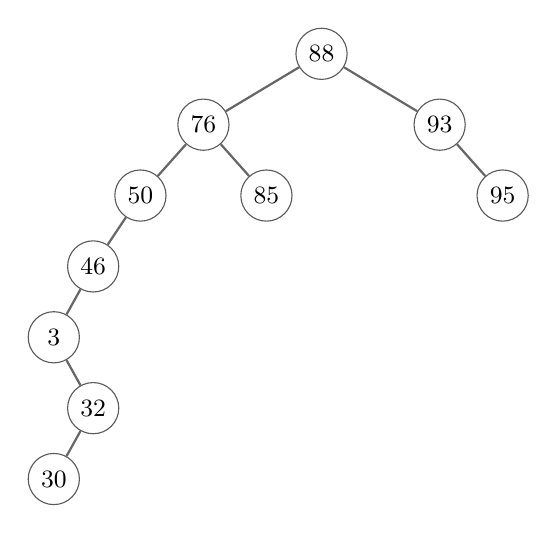
\begin{tikzpicture}[
    tn/.style={circle, draw=black!65, line width=0.4pt, minimum size=6.5mm, inner sep=0pt, font=\small},
    level distance=9mm, edge from parent/.style={draw=black!60, thick},
    level 1/.style={sibling distance=30mm}, level 2/.style={sibling distance=16mm},
    level 3/.style={sibling distance=12mm}, level 4/.style={sibling distance=10mm},
    level 5/.style={sibling distance=10mm}, level 6/.style={sibling distance=10mm}]
\node[tn] {88}
    child {node[tn] {76}
        child {node[tn] {50}
            child {node[tn] {46}
                child {node[tn] {3}
                    child[missing]
                    child {node[tn] {32}
                        child {node[tn] {30}}
                        child[missing]}}
                child[missing]}
            child[missing]}
        child {node[tn] {85}}}
    child {node[tn] {93}
        child[missing]
        child {node[tn] {95}}};
\end{tikzpicture}
\end{center}
最長的路徑是 $88 \to 76 \to 50 \to 46 \to 3 \to 32 \to 30$，$7$ 個節點、$6$ 條邊。 高度數邊是 $6$，選 (B)；
資結書的高度數節點（資結書第~9~章開頭），那樣是 $7$，會選 (C)。 (A) 4 是 $10$ 個節點平衡時
（數邊 $\lfloor \lg 10 \rfloor = 3$、數節點 $4$）才有的高度；(D) 8 兩種定義都不對。

\textbf{14. 刪除 $76$。} $76$ 有兩個子節點 $50$、$85$，用後繼取代：右子樹 $\{85\}$ 的最小值是 $85$，
它沒有左子節點，直接頂替 $76$ 的位置，$50$ 成為 $85$ 的左子節點。 所以 $50$ 的父節點是 $85$，
選 (B)。 改用前驅（左子樹最大，這裡是 $50$ 本身，它沒有右子節點）的話，$50$ 頂替 $76$，父節點變
成 $88$，會選 (C)。 這種有兩種合理做法的題目，作答時要寫出用的是後繼。 (A) 46 是 $50$ 的子節點，
(D) 93 在另一邊，兩種做法都不會是。

\textbf{15. AVL 樹。} 每次插入後從新節點往上找第一個不平衡（左右子樹高度差 $2$）的節點，依形狀
旋轉（資結書第~10.2.3~節）：
\begin{center}
\footnotesize\setlength{\tabcolsep}{4pt}
\begin{tabular}{rll}
\toprule
插入 & 發生的事 & 之後的樹（根(左, 右)） \\
\midrule
88, 93, 76 & 都平衡 & $88(76, 93)$ \\
50 & 平衡 & $88(76(50, \cdot), 93)$ \\
46 & $76$ 不平衡，LL，在 $76$ 右旋 & $88(50(46, 76), 93)$ \\
3 & $88$ 不平衡，LL，在 $88$ 右旋 & $50(46(3, \cdot), 88(76, 93))$ \\
32 & $46$ 不平衡，LR，$3$ 左旋、$46$ 右旋 & $50(32(3, 46), 88(76, 93))$ \\
85 & 平衡 & $50(32(3, 46), 88(76(\cdot, 85), 93))$ \\
30 & 平衡 & $50(32(3(\cdot, 30), 46), 88(76(\cdot, 85), 93))$ \\
95 & 平衡 & $50(32(3(\cdot, 30), 46), 88(76(\cdot, 85), 93(\cdot, 95)))$ \\
\bottomrule
\end{tabular}
\end{center}
插入 $3$ 那一步要注意：從 $3$ 往上，$46$ 的左右高度差是 $1$、$50$ 是 $2 - 1 = 1$，第一個差 $2$ 的是
$88$（左子樹 $50(46(3), 76)$ 高度 $3$，右子樹 $93$ 高度 $1$），$3$ 在 $88$ 的左子節點 $50$ 的左子樹裡，
是 LL。 最後的樹：
\begin{center}
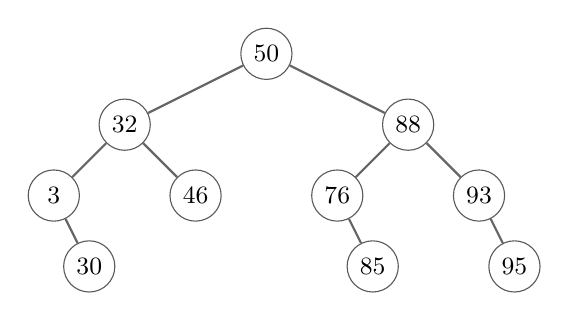
\begin{tikzpicture}[
    tn/.style={circle, draw=black!65, line width=0.4pt, minimum size=6.5mm, inner sep=0pt, font=\small},
    level distance=9mm, edge from parent/.style={draw=black!60, thick},
    level 1/.style={sibling distance=36mm}, level 2/.style={sibling distance=18mm},
    level 3/.style={sibling distance=9mm}]
\node[tn] {50}
    child {node[tn] {32}
        child {node[tn] {3} child[missing] child {node[tn] {30}}}
        child {node[tn] {46}}}
    child {node[tn] {88}
        child {node[tn] {76} child[missing] child {node[tn] {85}}}
        child {node[tn] {93} child[missing] child {node[tn] {95}}}};
\end{tikzpicture}
\end{center}
$76$ 的父節點是 $88$，選 (C)。 (A) 46 在根的左子樹裡，(B) 85 是 $76$ 的子節點，(D) 93 是 $76$ 的兄弟。

\textbf{16. 刪除 $32$。} $32$ 有兩個子節點，用後繼 $46$（右子樹的最小值，是葉節點）取代，再刪掉原本
的 $46$。 這時頂替上來的節點 $46$ 左子樹是 $3(\cdot, 30)$（高度 $2$），右子樹是空的，不平衡；左子節點
$3$ 是右邊比較高，屬於 LR（資結書第~10.2.6~節）：先在 $3$ 左旋得 $30(3, \cdot)$，再在 $46$ 右旋，
這棵子樹變成 $30(3, 46)$。 往上到根 $50$：左高 $2$、右高 $3$，平衡。 結果：
\[
50\bigl(30(3, 46),\; 88(76(\cdot, 85), 93(\cdot, 95))\bigr),
\]
$30$ 的父節點是 $50$，選 (C)。 改用前驅 $30$ 取代 $32$ 也一樣：$30$ 頂替 $32$，刪掉原本的 $30$ 後
子樹是 $30(3, 46)$，平衡，父節點同樣是 $50$。 (A) 3 是刪除前 $30$ 的父節點；(B) 46、(D) 76 都不是。
\end{pastsoln}
